\thesischapterexordium

\section{基于电磁学的神经成像}
\subsection{脑电研究方法进展}
根据脑电的产生,发展和广泛应用,以及随着材料、采集技术、计算机技术的发展,脑电研究方法分为四个阶段:视觉分析、纸质统计分析、计算机辅助分析、高性能分析。其中在1980年,ER John提出了定量脑电概念。根据脑电分析方法类型,分为标准化去伪差、头表源空间、时空频、谱网络、线性非线性、回归学习预测等。脑电分析方法还有多模态融合,在心理学、脑疾病和工程领域得到应用。

\begin{figure}
	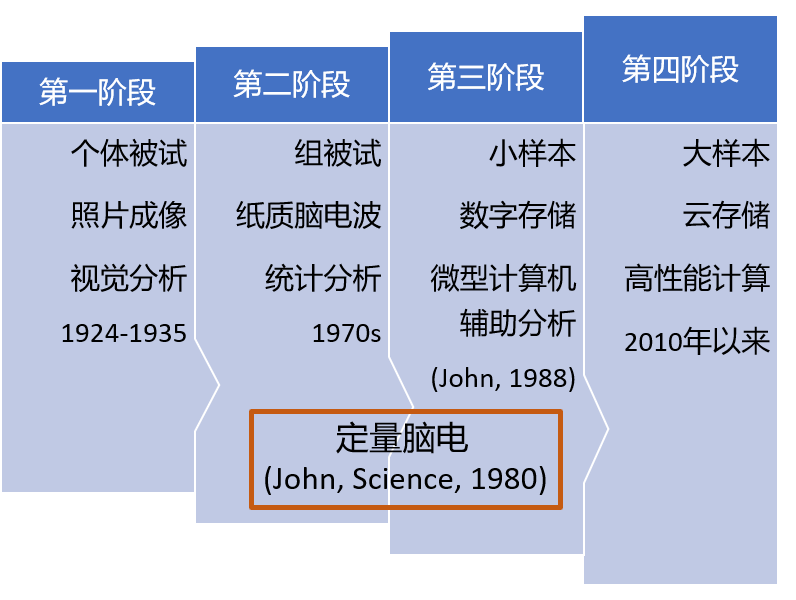
\includegraphics[width=15cm]{pic/xulun/figure1.png}
	\caption{脑电研究方法进展}
\end{figure}
%\subsection{脑磁图}
%\subsection{核磁共振成像}
%\subsection{模态之间的联系}

\begin{figure}
	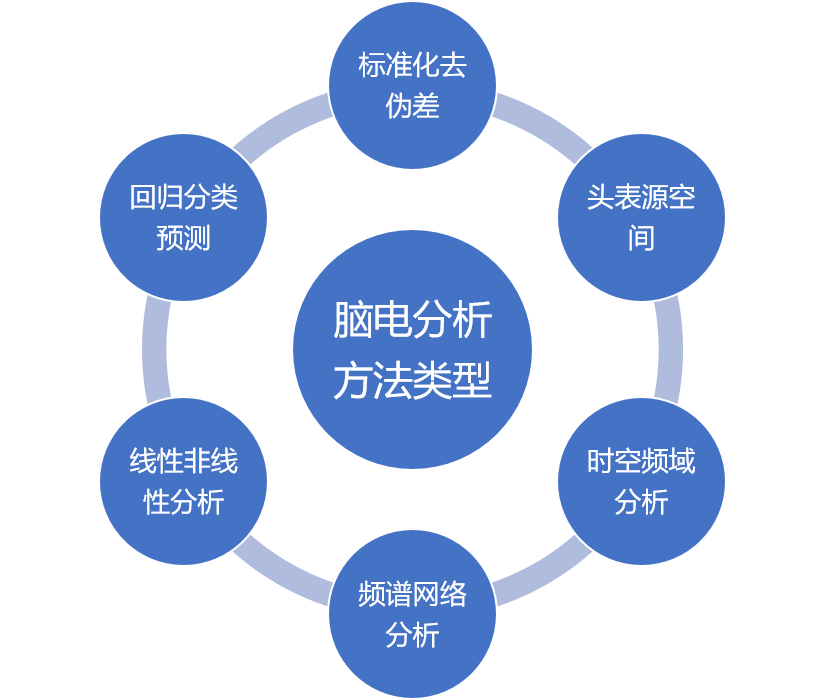
\includegraphics[width=15cm]{pic/xulun/figure2.png}
	\caption{脑电研究方法分类}
\end{figure}

\section{定量脑电}
Berger在记录人类头表脑电的实验中也认识到了,参考电极问题。 Berger对脑电波形的分析中,认识到了alpha波和beta波,频域分析的开始。
参考电极影响波形,频域分析等等。 定量脑电就是基于静息态脑电数据的频谱特征分析、常模估计、预测诊断等等。
定量脑电是基于静息态脑电谱特征的诊断方法,谱特征与正常值的偏差可以通过正常脑电数据库年龄因素调整后的谱特征的均值和标准偏差的z变换来判定测量。

\section{下一代定量研究方法}
当前的脑电数据分析具有一些存在的问题:
随着高性能计算、统计学习的进展,下一代定量脑电分法来临,主要是多样的数据格式 到BIDS标准,多种参考到参考标准化,小样本常模到国际通用的常模,以及神经震荡多谱峰节律分析,从单变量谱到多变量交叉谱,从多变量欧式空间 到 协方差黎曼流形统计等等。
\begin{figure}
	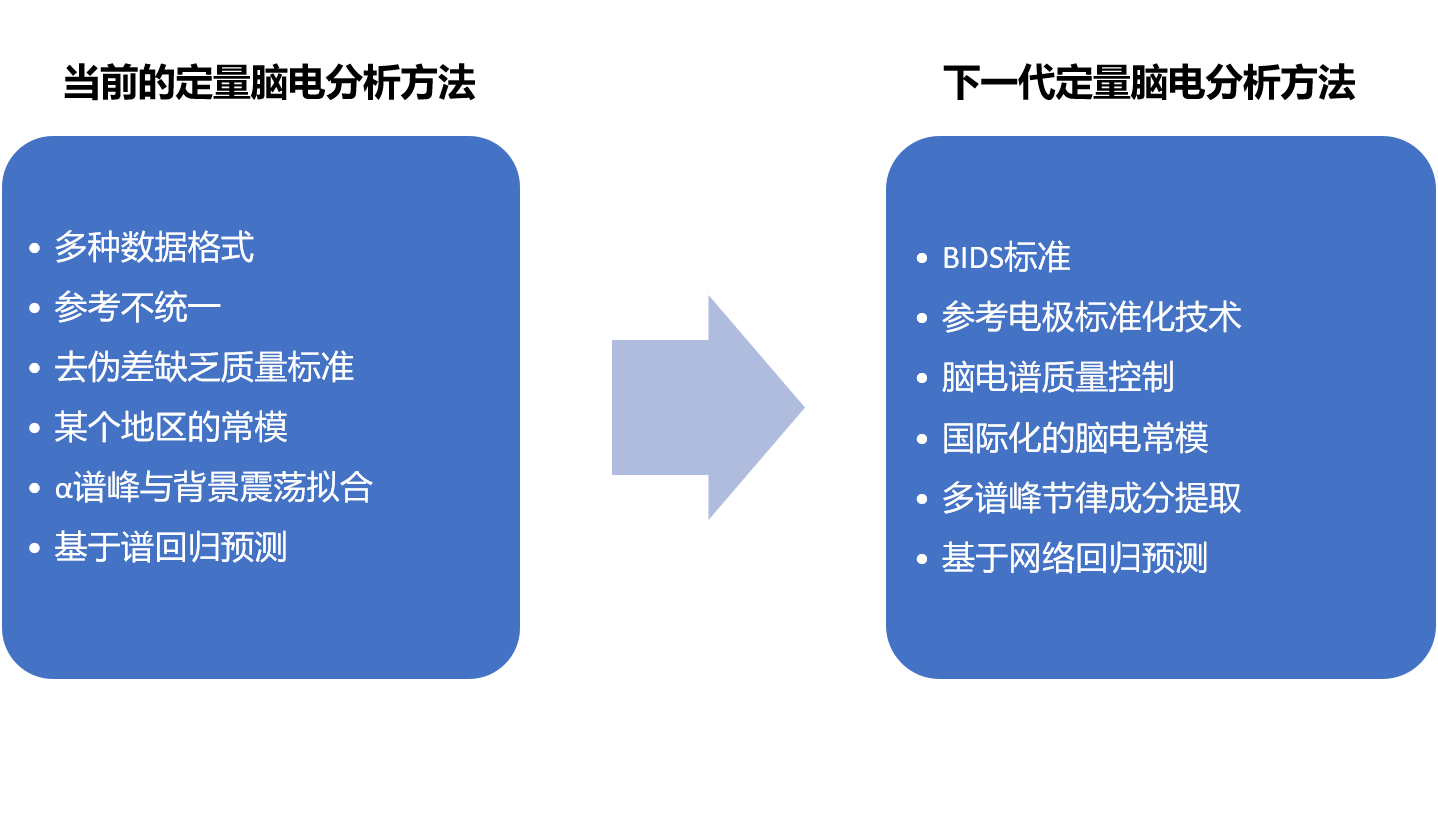
\includegraphics[width=15cm]{pic/xulun/figure3.png}
	\caption{当前和下一代定量脑电分析方法}
\end{figure}
\section{本文拟解决的问题}
从物理或实际数据采集的角度,参考如何受到综合多种因素的影响。
把参考看作模型,是否能够从统计学习的角度进行参考选择。
不同参考物理假设的数学证据,参考的内在联系和属性是什么。
大量脑电谱分析的自动质量控制准则是什么。
不同国家或被试群体之间是否存在一致的脑电谱常模演化曲线?
脑电定量谱分析、多重节律成分的合理方法。

\section{本文的主要贡献与创新}
本论文以定量脑电技术中的无穷远参考、贝叶斯估计、大样本脑电谱筛选准则、谱常模回归、协方差的结构为重点研究内容,主要创新点与贡献如下:
1. 从参考的物理学假设出发,综合分析了参考模态和电极配置等多种因素对参考在脑电电位记录信号误差的影响,这些因素包括:从稀疏到致密的具有不同电极数目的电极配置、

\section{本论文的结构安排}
本文的章节结构安排如下:
\begin{description}
	\item[第一章] 绪论。
	\item[第二章] 以参考电极和电极配置为重点讲述定量脑电中电势的影响因素。
	\item[第三章] 主要描述了脑电无穷远参考的统一的贝叶斯统计学架构。
	\item[第四章] 描述了单点参考的统计学推导和属性以及综合讨论在实际应用中注意事项。
	\item[第五章] 描述了大样本脑电谱的同构异质性研究
	\item[最后一章] 总结与展望
\end{description}
